% (c) 2020 Stefan Antonowicz
% Based off of tex found at https://github.com/ludus-leonis/nipajin
% This file is released under Creative Commons Attribution-NonCommercial-ShareAlike 4.0 International License.
% Please do not apply other licenses one-way.

\renewcommand{\yggPhilosophers}{%
  \mychapter{Philosophers}{philosophers}
}

\renewcommand{\yggPhilosophersText}{%

 \mysection{The Crux of Blood}{philosopher-crux-blood}

 The Crux of Blood grants the Philosopher a Blood Die - a d6 \POOL used to perform \mylink{Wizardry}{arcana-wizardry}.  When you first learn the Crux of Blood, choose a \mylink{Wizardry}{philosopher-wizardry} spell.  This spell is etched on the inside of your cranium "...like moth larvae burrowing through the bark of a tree."  This spell can be cast without speaking or moving.  If someone cuts off your head and scoops out your brains, they can read (and learn) the spell too (see \mylink{Fetishes}{philosopher-fetishes}).


\mysubsection{Wizardry}{philosopher-wizardry}

Performing Wizardry requires rolling one or more Blood Die - how many is up to you, but you have to roll them all at once.  Each Blood Die is a \POOL; if you roll a 1 or a 2 on a Blood Die, you lose the die. Additionally:

\mybullet {
  \item If you roll any triples, roll on the \mylink{Mishap table}{table-mishap}. The spell works.
  \item If you roll any quadruples, roll on the \mylink{Calamity table}{table-calamities}. The spell fails.
  \item If you roll any quintuples, roll on the \mylink{Ruin table}{table-ruin}. The spell fails.  This will most likely kill you.
}


You restore 1 Blood Die when you Bivouac, or all your Blood Die with a Vacation - but you can also attempt to ride the Torrent.

More information on Wizardry and spells can be found in the section on \mylink{Arcana}{arcana-wizardry}

\mysubsection{The Torrent}{philosopher-torrent}

If you have 0 Blood Die in your pool, you can try to cast your Wizardry directly from the Torrent (a dangerous proposition).  For each Blood Die you want to add to your Wizardry, try the following \RO:

\example {
  \mybold{Torret}

  \RO : \INT plus d6 plus Modifiers ~\\ ~\\

  \myital{Don't forget to add your \LVL, since this roll uses your \INT!}
}

If you succeed, you can add a Blood Die to the spell.  You can do this as many times as you like for each spell. If you fail any \RO attempt, the spell fails and you suffer a \mylink{Calamity}{table-calamities}.

  \begin{center}
  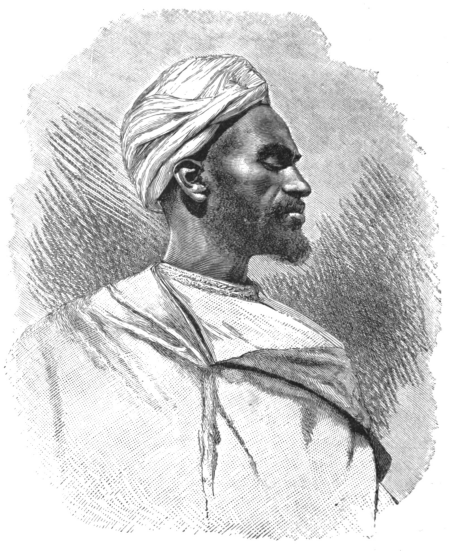
\includegraphics[scale=.5]{Philosopher_1}
  \end{center}


\mysubsection{Components}{philosopher-components}

You can harvest and use components to cast spells:

\example {
  \mybold{Harvest Component}
  \RO : \INT plus d6 plus d20 plus Modifiers

  ~\\
  
  \myital{Don't forget to add your \LVL, since this roll uses your \INT!}
}

If you succeed on your \RO try, gain d4 \UD of a Component.

You decide what Components augment which spells. For example, you could declare that kobold's eyes are a component for the spell Sleep.  If you succeed in your \RO try, then kobold's eyes are always a component for Sleep (note it on your character sheet) for YOU and not for anyone else (someone else's version of Sleep has a different way of casting, needs boggart boogers or whatever). 

If you cast a spell with a Component, then you only burn a Blood die if you roll a 1 (instead of a 1 or 2).  Components are Insignificant items, but using a component consumes it in a puff of smoke / blue flame / swarm of gnats etc.

\mybullet {
  \item Components can only be harvested during a Breather, and have to be from one of the Monsters you've (presumably) killed.  It has to be something you can reasonably carry (Arbiter's choice) - basilisk tongue, ok.  Green slime, not ok.
  \item Monsters only provide one component.  You can't say kobold's eyes help Magic Missile and kobold's tongues help cast Battering Beam.   
  \item You can only try once per Monster type per Breather, so if you kill 9 kobolds and 14 trolls then you get two shots - once on kobolds and once on trolls.
  \item You can only harvest d4 \UD from a Monster no matter how many there are - 9 kobolds or 1, you get d4 \UD
}


\mysubsection{Grimoires}{philosopher-grimoires}

Grimoires are solid, with thick vellum pages and a sturdy cover. Special runes and symbols trap spells inside cages of crystallized thought. Each book contains enought room for 10 spells. Some spells must be stored across several pages for safety, so the books contain more than 10 pages, and have
plenty of room for notes, ledgers, or sketches - and curses, hexes, coded and cryptic entries written with poisonous and hallucinogenic inks. Grimoires start in a waterproof, acid- and fire-resistant bag. Outside the bag, they are not waterproof and are quite flammable. See the section on
\mylink{Inscription}{research-inscription} for more details.


\mysubsection{Fetishes}{philosopher-fetishes}

Fetishes are inscribed with a single spell from your grimoire, cranium, or another fetish.  All fetishes have a \UD of d4 - when the \UD is exhausted, the magical words disappear from the fetish.  A Sorcerer's skull counts as a fetish, though obviously the brain can't be in the way if you want to read
it.  See the section on \mylink{Inscription}{research-inscription} for more details.

You may cast the spell from the Fetish with any number of Blood you choose, OR you may forgo the Blood die and roll a single d6 for the effect.

\mysubsection{Wizards' Duel}{philosopher-wizards-duel}

Certain spells can be countered by other spells - for example,
\mylink{Balthazar's Breathtaking
Blast}{wizardry-balthazars-breathtaking-blast} can be countered by
\mylink{Mighty Lungs}{wizardry-mighty-lungs}, and
\mylink{Invisibility}{wizardry-invisibility} can be dispelled by the wisps
summoned in the \mylink{Fool's Fire}{wizardry-fools-fire} spell. 

If you attempt to counter a spell and the Sorcerer who cast it is not
present (that is, not somewhere Close, Nearby, Far-Away, or Distant) you
automatically succeed.  Otherwise, you enter into a duel with the other
Sorcerer.

Each Sorcerer must \RB : \INT, adding their \LVL and the \DICE invested in
the spell as well as any other modifiers.  

\example {
  \mybold{A Wizards' Duel is}
  \RB : \INT plus \LVL plus \DICE
}


The winner's spell stays, the loser's spell goes.  Put another way: 

\mybullet{
  \item If you are countering a spell and you win, the spell you're
attempting to counter is dispelled and your spell takes effect
  \item If you are countering a spell and you lose, the spell you're
attempting counter remains and your spell fizzles with no effect.
}

If you attempt to counter a spell and you roll a \mylink{Calamity}{table-calamities} or \mylink{Ruin}{table-ruin}, the counterspell doesn't work. 


\newpage




\end{multicols}

 \mysection{The Crux of Knowledge}{philosopher-crux-knowledge}

\begin{multicols}{2}\raggedbottom

  
  The Crux of Knowledge gives you a \STATIC Knowledge Die that you can use to learn and practices the sciences, most notably Leechcraft.  The Crux of Knowledge bestows an honorific on the practioner; your title will be used in "polite society".   


    \mytable{X r}{
      \thead{Honorific} & \thead{Knowledge Die} \\
    }{
      Honorable & d10 \STATIC \\
      Professor & d12 \STATIC \\
      Doctor & d16 \STATIC \\
      Maestro & d20 \STATIC \\
    }

   


\mysubsection{Leechcraft}{philosopher-leechcraft}

Knowledge Dice are used in the pratice of \mylink{Leechcraft}{arcana-leechcraft}.   In order to perform the healing arts, you must roll your Knowledge Die vs. a Target.  Your \INT adds a bonus to your roll:

    \mytable{X r}{
      \thead{\INT} & \thead{Bonus} \\
    }{
      d2-d10 & +0  \\
      d12 & +1  \\
      d16 & +2  \\
      d20 & +3  \\
      d24 & +4 \\
    }
   
  When applying Leechcraft, if you roll less than the Target number, your next roll is at -2.  This is cumulative:  -2 for the first miss, -4 for the second, etc.  These negatives are removed when you take a Bivouac.

  \begin{center}
  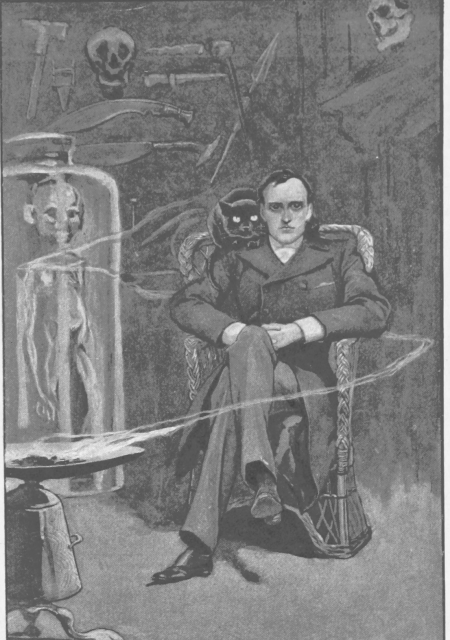
\includegraphics[scale=.5]{Philosopher_2}
  \end{center}


\mysection{Research}{philosopher-research}


Research can be gained by learning Chymistry, Medicinals, or Inscription.  It is used during a Vacation, and be used to help Spriggans create magic weapons. 




} % end
